\documentclass[aspectratio=169]{beamer}

% because we need to claim weird things
\newtheorem{claim}{Claim}
\newtheorem{defn}{Definition}
%\newtheorem{lemma}{Lemma}
\newtheorem{thm}{Theorem}
\newtheorem{vita}{Vit\ae}
\newtheorem{qotd}{Quote of the Day}

\usepackage{algorithm}
\usepackage{algpseudocode}
\usepackage{listings}
\usepackage{color}
\usepackage{graphics}
\usepackage{ulem}
\bibliographystyle{unsrt}

% background image
\usebackgroundtemplate%
{%
    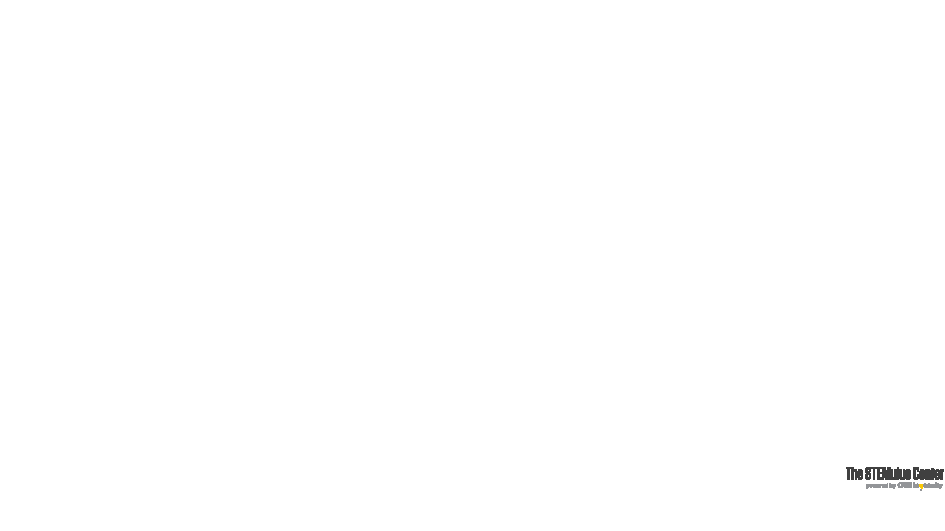
\includegraphics[width=\paperwidth,height=\paperheight]{../artifacts/stemulus.pdf}%
}
\setbeamertemplate{caption}[numbered]
\lstset{%
	breaklines=true,
	captionpos=b,
	frame=single,
	keepspaces=true
}

% page numbers
\addtobeamertemplate{navigation symbols}{}{%
    \usebeamerfont{footline}%
    \usebeamercolor[fg]{footline}%
    \hspace{1em}%
    \insertframenumber/\inserttotalframenumber
}

% presentation header
\usetheme{Warsaw}
\title{Week 1: HTML Review}
\author{Dylan Lane McDonald}
\institute{CNM STEMulus Center\\Web Development with PHP}
\date{\today}

\begin{document}
\lstset{language=HTML}
\begin{frame}
\titlepage
\end{frame}

\begin{frame}
\frametitle{Outline}
\tableofcontents
\end{frame}

\section{HTML Tags}
\subsection{Tags}
\begin{frame}
\frametitle{HTML Tags}
An HTML \textbf{tag} defines a behavior within an HTML document and represents an individual component of the HTML document. All the HTML tags are then parsed into the HTML Document Object Model (DOM).
\pause
\begin{defn}
The \textbf{Document Object Model (DOM)} is a hierarchical representation of an HTML document. The DOM hierarchy allows other software (e.g., parsers) and languages (e.g., JavaScript) to access the HTML document.
\end{defn}
\end{frame}

\begin{frame}
\frametitle{Common HTML Tags}
\begin{qotd}
Seeing, hearing, feeling, are miracles, and each part and tag of me is a miracle.\\
$\approx$ Walt Whitman
\end{qotd}
\pause

Common HTML tags include:
\begin{itemize}
	\item \texttt{<p>}: paragraph
	\item \texttt{<br />}: line break
	\item \texttt{<strong>}: bold
	\item \texttt{<body>}: document body
	\item Many more; use a cheat sheet! \cite{cheatography, w3schools}
\end{itemize}
\end{frame}

\subsection{HTML Tag Attributes}

\begin{frame}
\frametitle{HTML Tag Attributes}
An HTML attribute modifies the behavior of an HTML tag. Attributes are typically in name/value pairs and are separated by a ``='' character after the tag's name:

\pause
\mbox{}\\
\texttt{<tag attribute1="value" attribute2="value"> (content within this tag)</tag>}

\pause
\mbox{}\\
A tag can have as many attributes as necessary.
\end{frame}

\begin{frame}
\frametitle{Common Attributes}
Attributes vary by tag and are \textbf{NOT} universal, but some common attributes that appear for multiple tags are:
\begin{itemize}
	\item id: attribute for accessing the tag using JavaScript
	\item height: height of this object
	\item class: CSS style to apply to this tag
\end{itemize}
To find out all the possible attributes for a tag, use the W3C Cheatsheet. \cite{w3c}
\end{frame}

\section{Document Structure}
\subsection{Hi, World!}
\begin{frame}[fragile]
\frametitle{Shortest Possible HTML Document}
\begin{lstlisting}[caption=Shortest Possible HTML Document,label=code:html]
<!DOCTYPE html>
<html>
   <head>
       <title>Short HTML Document</title>
   </head>
   <body>
      <p>Short HTML Document</p>
   </body>
</html>
\end{lstlisting}
\end{frame}

\subsection{Document Hierarchy}
\begin{frame}
\frametitle{Indentation \& Code Style}
Notice the indentation of the tags in Listing \ref{code:html}. This is intentional. The purpose of the indentation is to:
\begin{enumerate}
	\item Increase readability by making it apparent to the reader what level the tag is at.
	\item Emphasize how deep or shallow in the hierarchy the tag is.
\end{enumerate}
For instance, the \texttt{<html>} tag will always be the shallowest tag in the hierarchy, since it indicates the beginning and ending of the HTML document. Conversely, the \texttt{<p>} tag is the deepest tag in the hierarchy in Listing \ref{code:html}.
\end{frame}

\begin{frame}
\frametitle{History of HTML}
HTML was developed at CERN by Tim Berners-Lee as a method of exchanging documents between locations.
\begin{vita}
\textbf{Tim Berners-Lee} invented HTML as a method of exchanging hypertext documents between servers. He wrote the first HTTP server and HTML client (browser) in 1990. He was knighted 2004 by Queen Elizabeth II and opened the London 2012 Olympics by tweeting ``This is for everyone'' to the audience and world.
\end{vita}
\end{frame}

\begin{frame}
\frametitle{Assignment}
Write an HTML page introducing yourself to the class. Use at least 10 different HTML tags in your document. Upload the resulting page to the students server and share it with the rest of the class.
\end{frame}

\begin{frame}
\frametitle{HTML Cheat Sheets}
\bibliography{html-tag-review}
\end{frame}

\end{document}